\documentclass[10pt]{beamer}

\usetheme[progressbar=frametitle]{metropolis}
\usepackage{appendixnumberbeamer}

\usepackage{booktabs}
\usepackage[scale=2]{ccicons}

\usepackage{pgfplots}
\usepgfplotslibrary{dateplot}

\usepackage{movie15}

\usepackage{xspace}
\newcommand{\themename}{\textbf{\textsc{metropolis}}\xspace}
\newcommand\nd{\textsuperscript{nd}\xspace}
\newcommand\rd{\textsuperscript{rd}\xspace}
\newcommand\nth{\textsuperscript{th}\xspace}

\usepackage{amsthm}
\usepackage{lineno}
\usepackage{amssymb,graphics,color,cite,amsmath}
\usepackage{wrapfig}

\usepackage{media9}%


\title{A Series of Experiments Based on Gyroscope}
\subtitle{2018}
\date{}
\author{Zeshun Zong and Yifeng Chen}
% tx392@nyu.edu}
\institute{Courant Institute of Mathematical Sciences, New York University}

\begin{document}

\maketitle

\begin{frame}[fragile]{Gyroscope}
\begin{figure}[h]
	\centering
	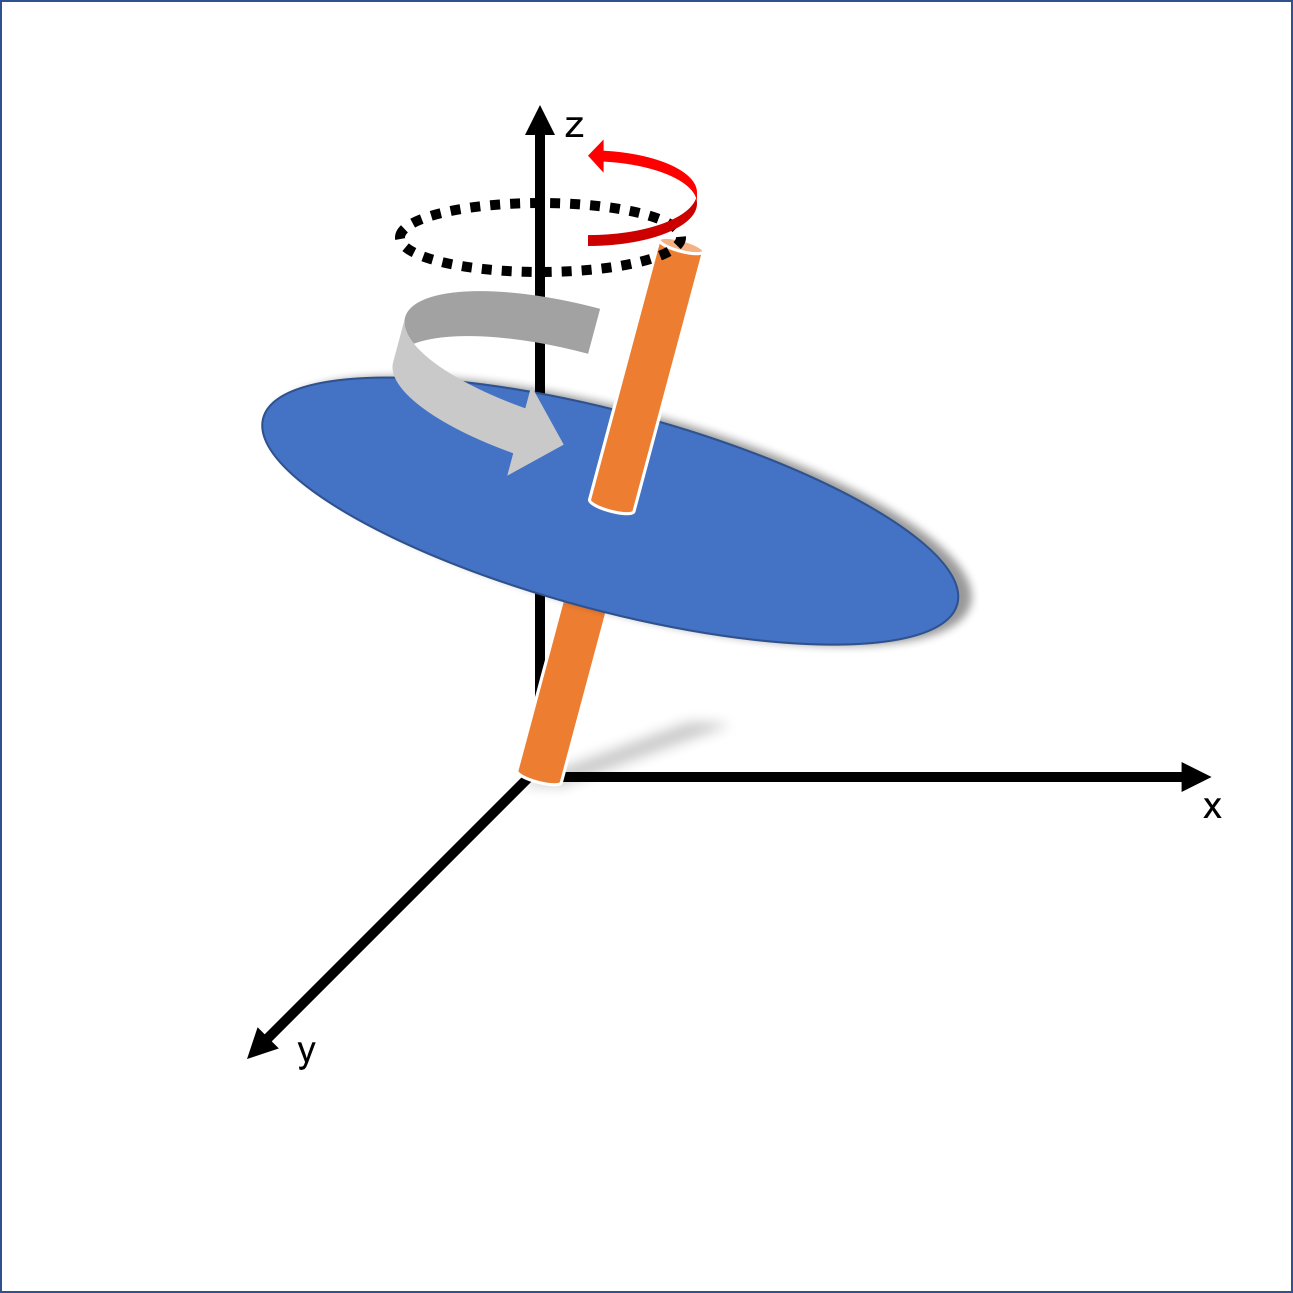
\includegraphics[width=0.6\textwidth]{sphere1.png}
\end{figure}

\end{frame}

\begin{frame}{Goal}
Gyroscope System: mass distribution and number of gyroscopes

Gyrocompass: how it works \& and analysis of its oscillation

\end{frame}

\section{Gyroscope System}

\begin{frame}{Parameters}
\begin{itemize}
\item dt
\item number of gyroscopes
\item spring constants
\item initial angular momentum L(0)
\item gravity
\item angle of inclination
\item stiffness of the ground
\item friction coefficient
\end{itemize}

\end{frame}


\begin{frame}{Algorithm}

    dL(t)/dt = \sum_k {\widetilde{X_k}}(t) \times F_k(t)
	
	L(t) = I(t)\omega(t) \hspace{5mm} where I(t) = \sum_k m_k [|{\widetilde{X_k}}(t)|^2 E - {\widetilde{X_k}} \cdot {\widetilde{X_k}}^T]
	
	\widetilde{X} = {P}(\Omega) \widetilde{X} + (E - {P}(\Omega)) \widetilde{X} \hspace{5mm} where P(\omega) = \frac{\Omega}{\|\Omega\|} \frac{\Omega^T}{\|\Omega\|} \widetilde{X}

\end{frame}


\begin{frame}{Standard Gyroscope}
    \begin{figure}
	\begin{minipage}{0.48\textwidth}
		\centering
		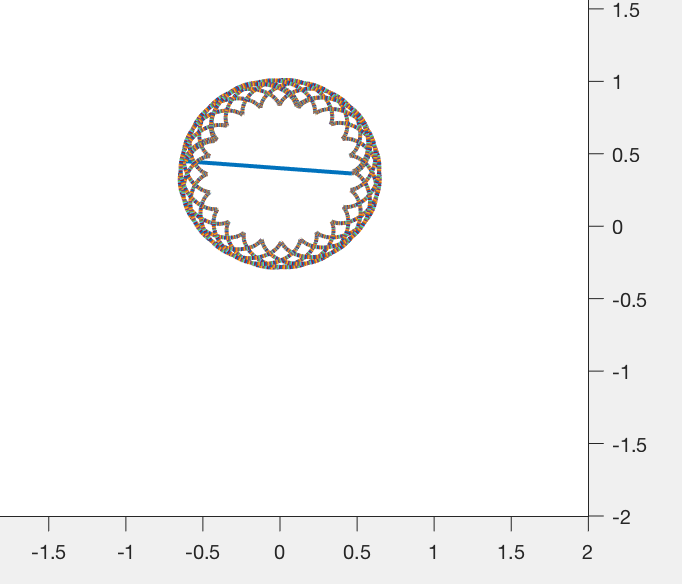
\includegraphics[width=\textwidth]{trace_even.png}
	\end{minipage}
    \end{figure}
\end{frame}

\begin{frame} {Uneven Mass Distribution}
    \begin{figure}
	\begin{minipage}{0.48\textwidth}
		\centering
		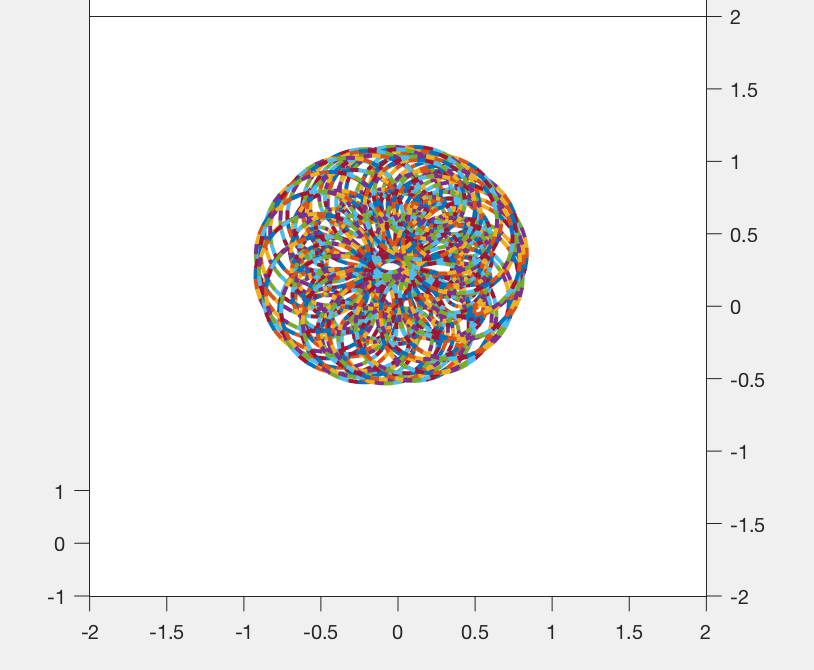
\includegraphics[width=0.8\textwidth]{trace_half.png}
	\end{minipage}
    \end{figure}
\end{frame}

\begin{frame} {Uneven Mass Distribution}
    \begin{figure}
	\begin{minipage}{0.48\textwidth}
		\centering
		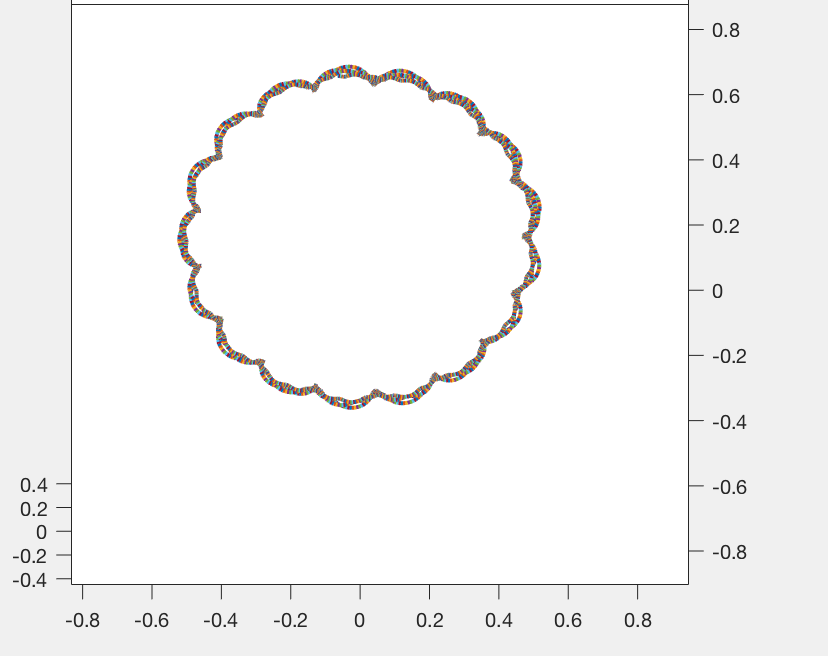
\includegraphics[width=0.8\textwidth]{trace_first5.png}
	\end{minipage}
	\begin{minipage}{0.48\textwidth}
		\centering
		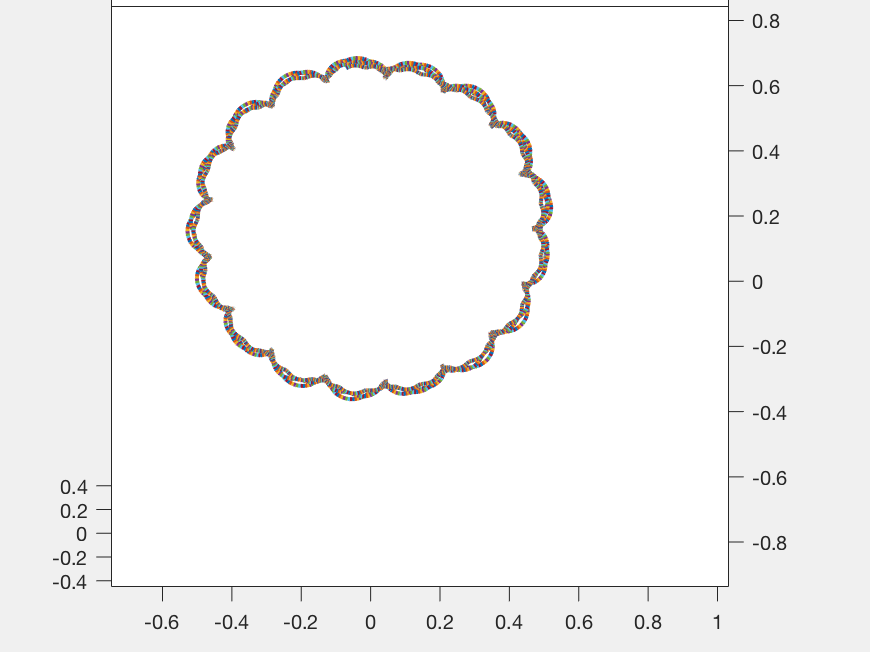
\includegraphics[width=0.8\textwidth]{trace_second5.png}
	\end{minipage}
    \end{figure}
\end{frame}

\begin{frame}{Multiple Gyroscopes}


\begin{figure}
	\begin{minipage}{0.48\textwidth}
		\centering
		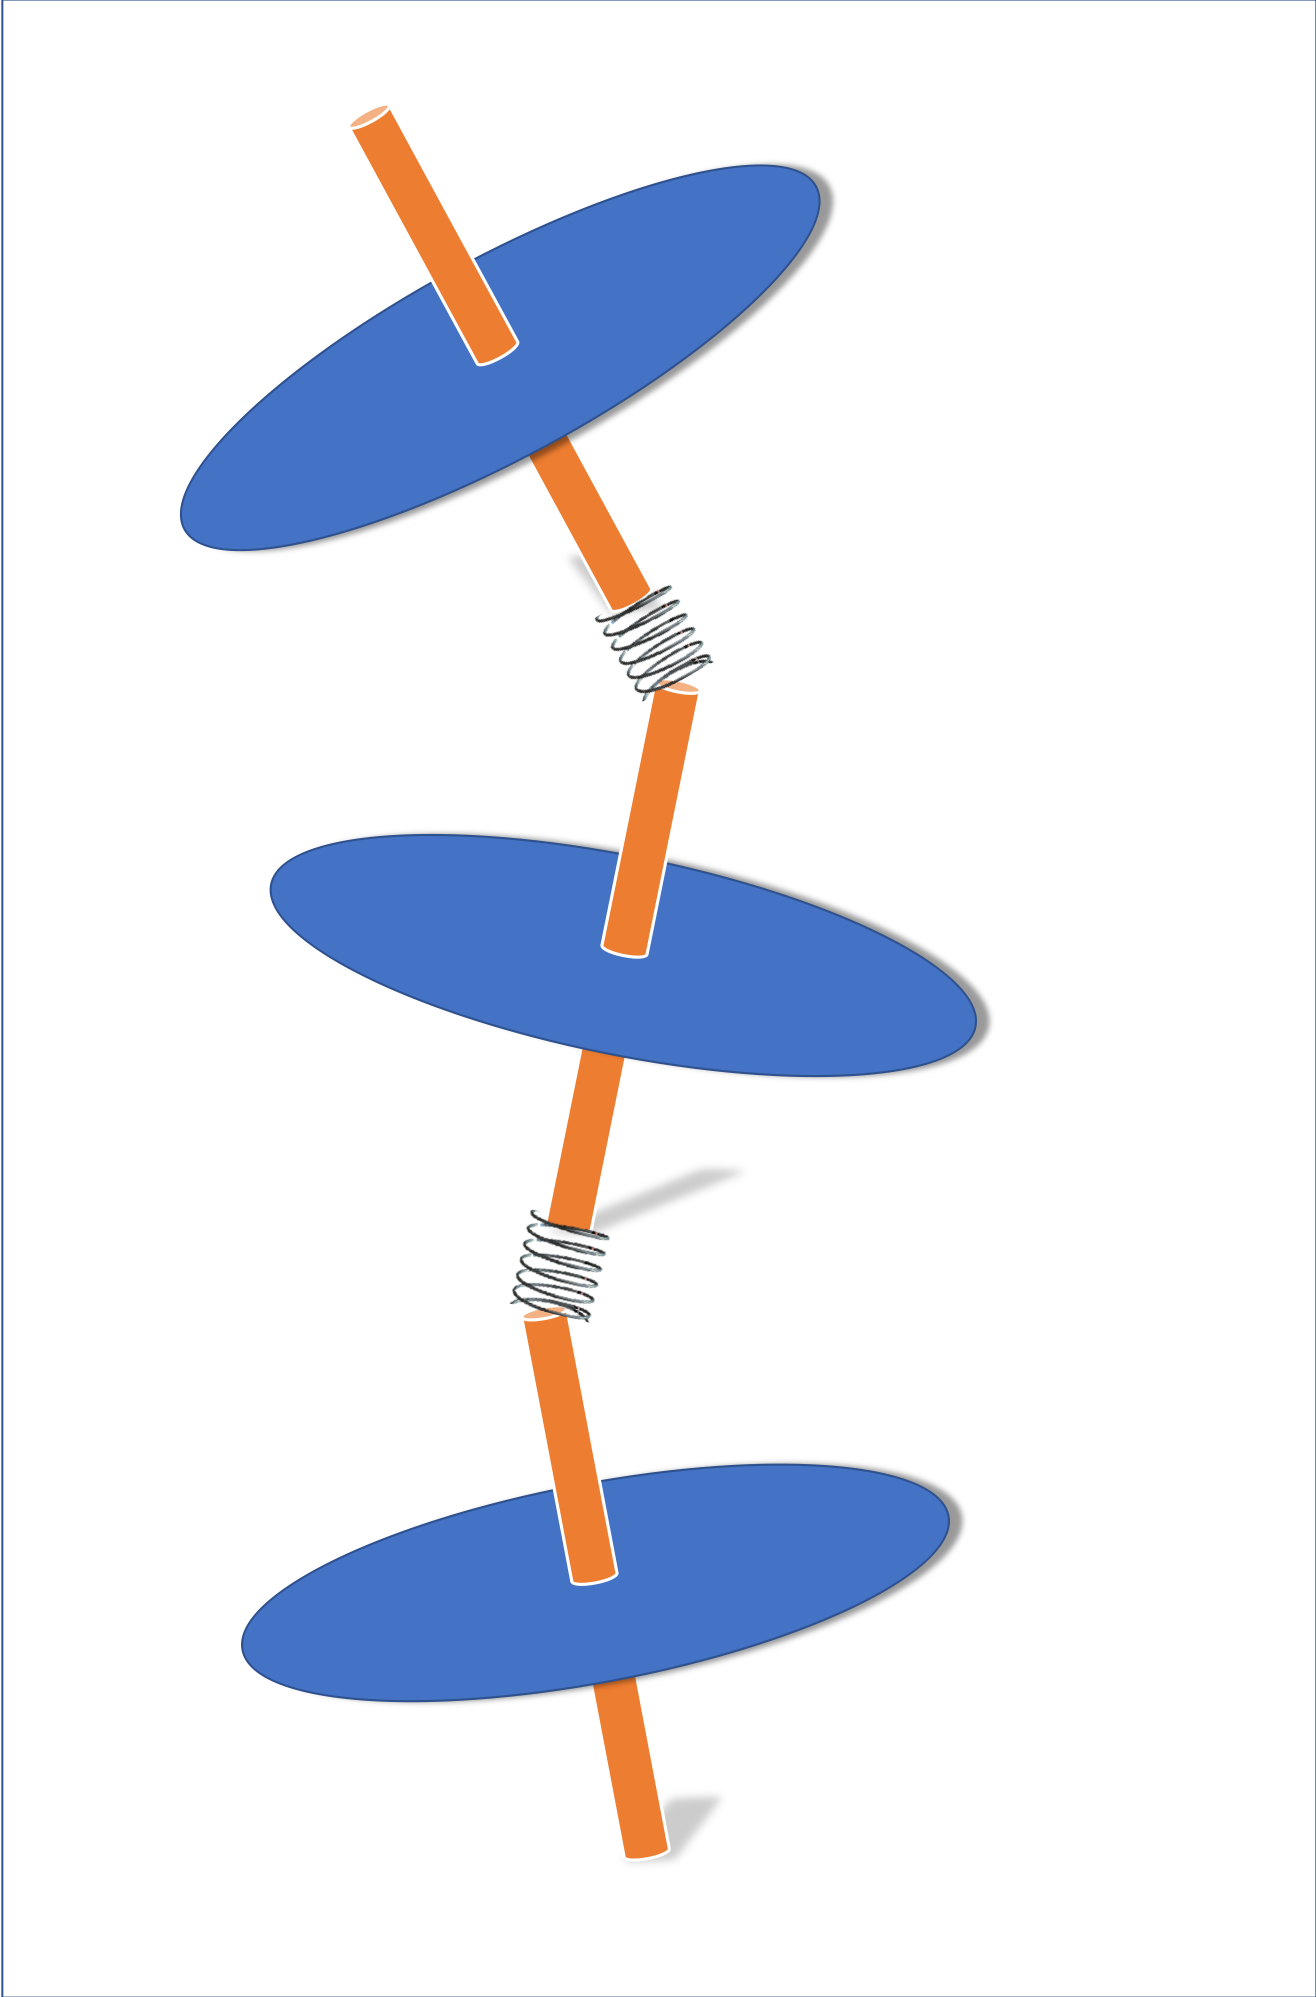
\includegraphics[width=\textwidth]{stack_model.png}
	\end{minipage}
\end{figure}

\end{frame}


\begin{frame}{Tests}

\end{frame}


\begin{frame}{Physics of Gyrocompass}
    \begin{figure}
		\centering
		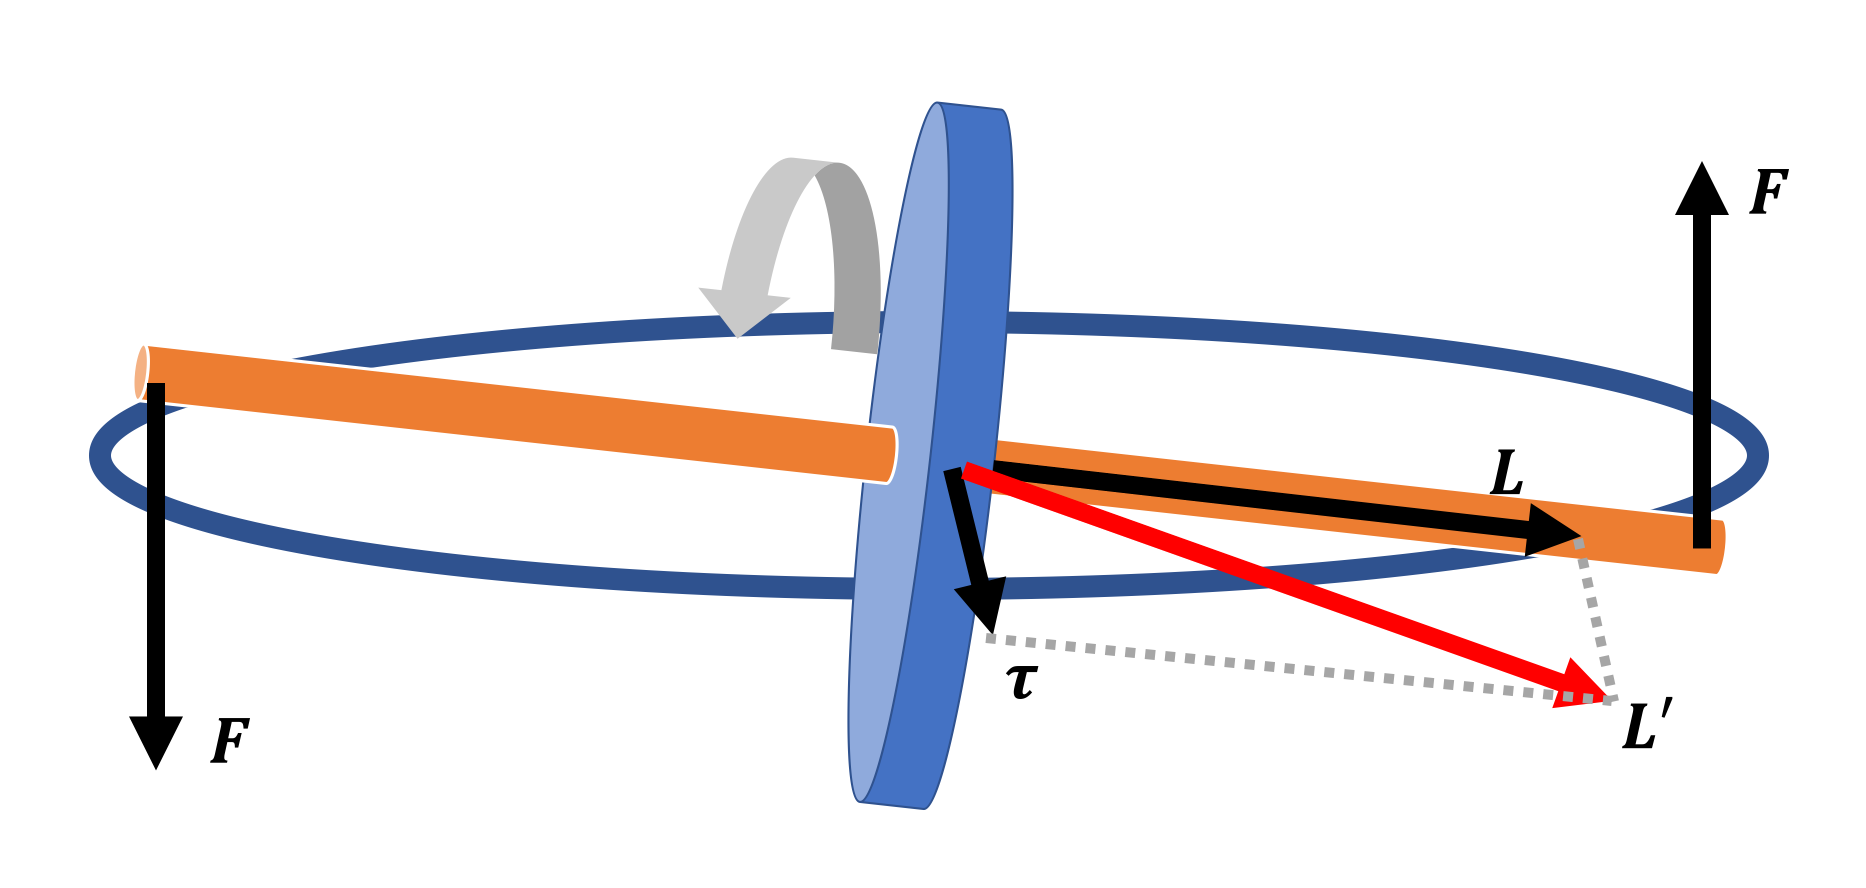
\includegraphics[width=\textwidth]{gyrocompass_physics.png}
	\end{figure}
\end{frame}

\begin{frame}{Set up}
\begin{figure}
		\centering
		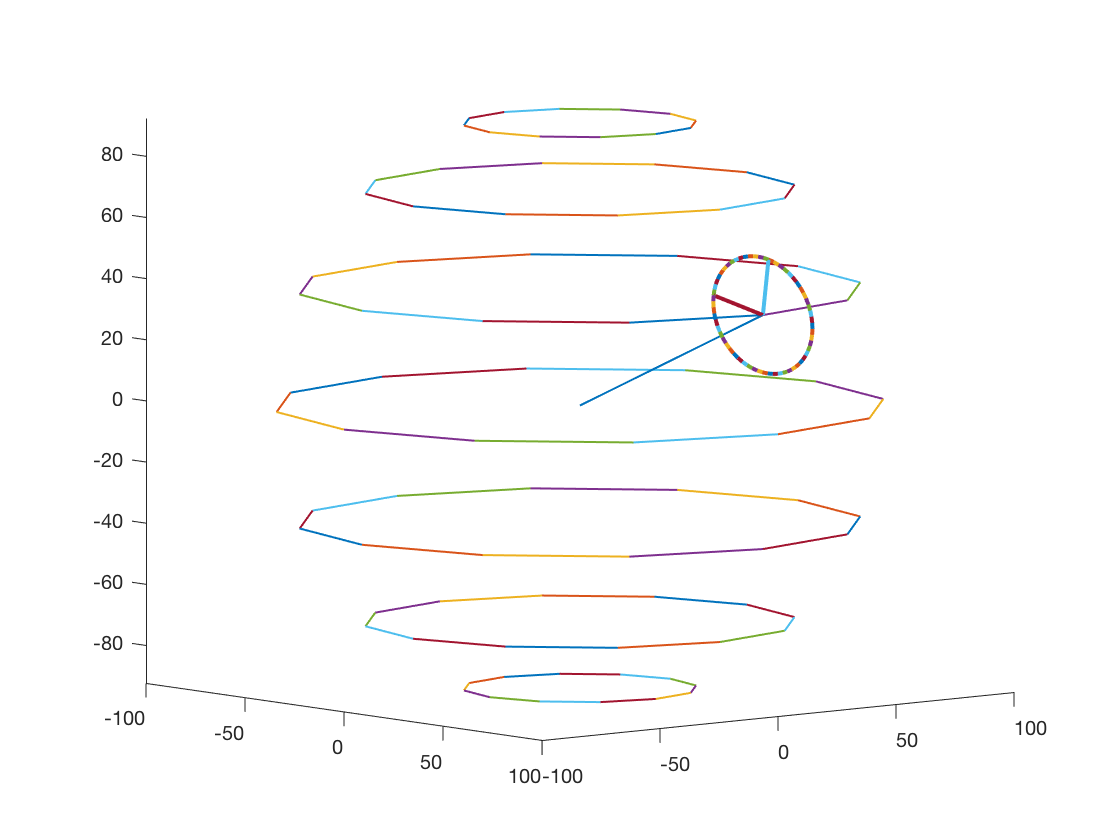
\includegraphics[width=\textwidth]{track_structure.png}
	\end{figure}
\end{frame}

\begin{frame}{Gyrocompass}
    \begin{figure}
		\centering
		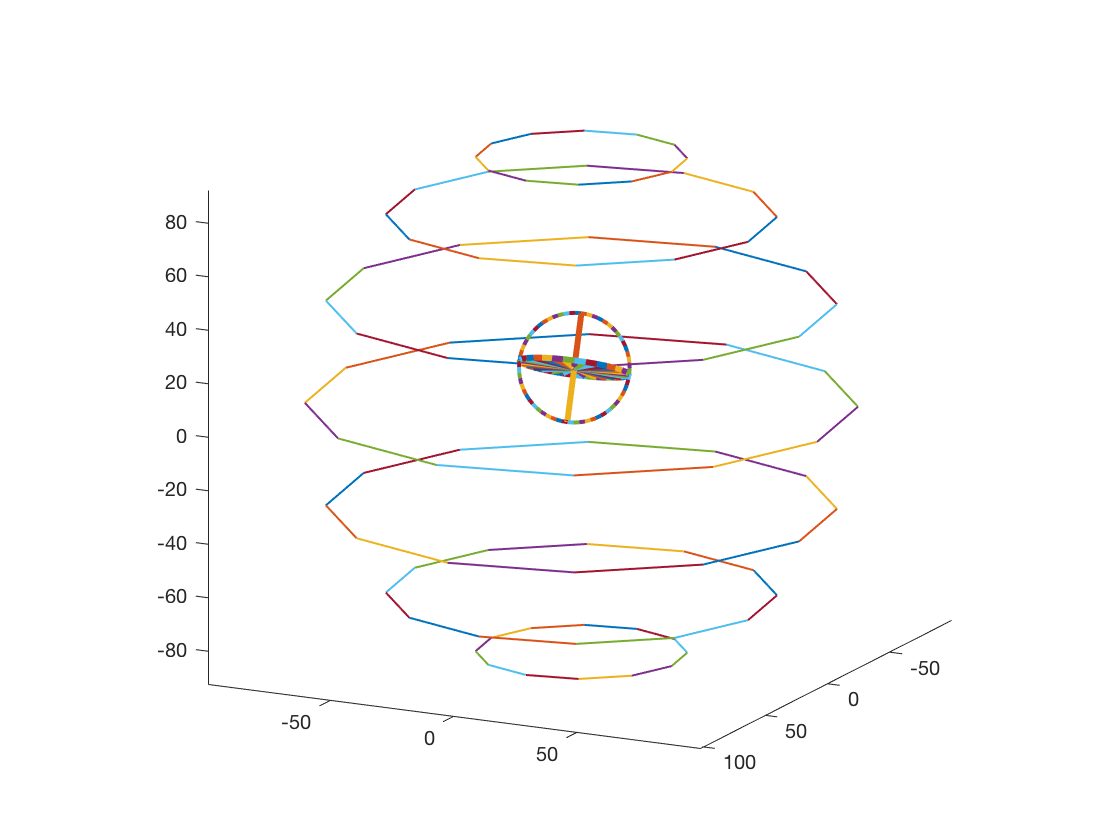
\includegraphics[width=\textwidth]{demo_pointing_north.png}
	\end{figure}
\end{frame}



\begin{frame}{Gyrocompass}
    \begin{figure}
    	
    		\centering
    		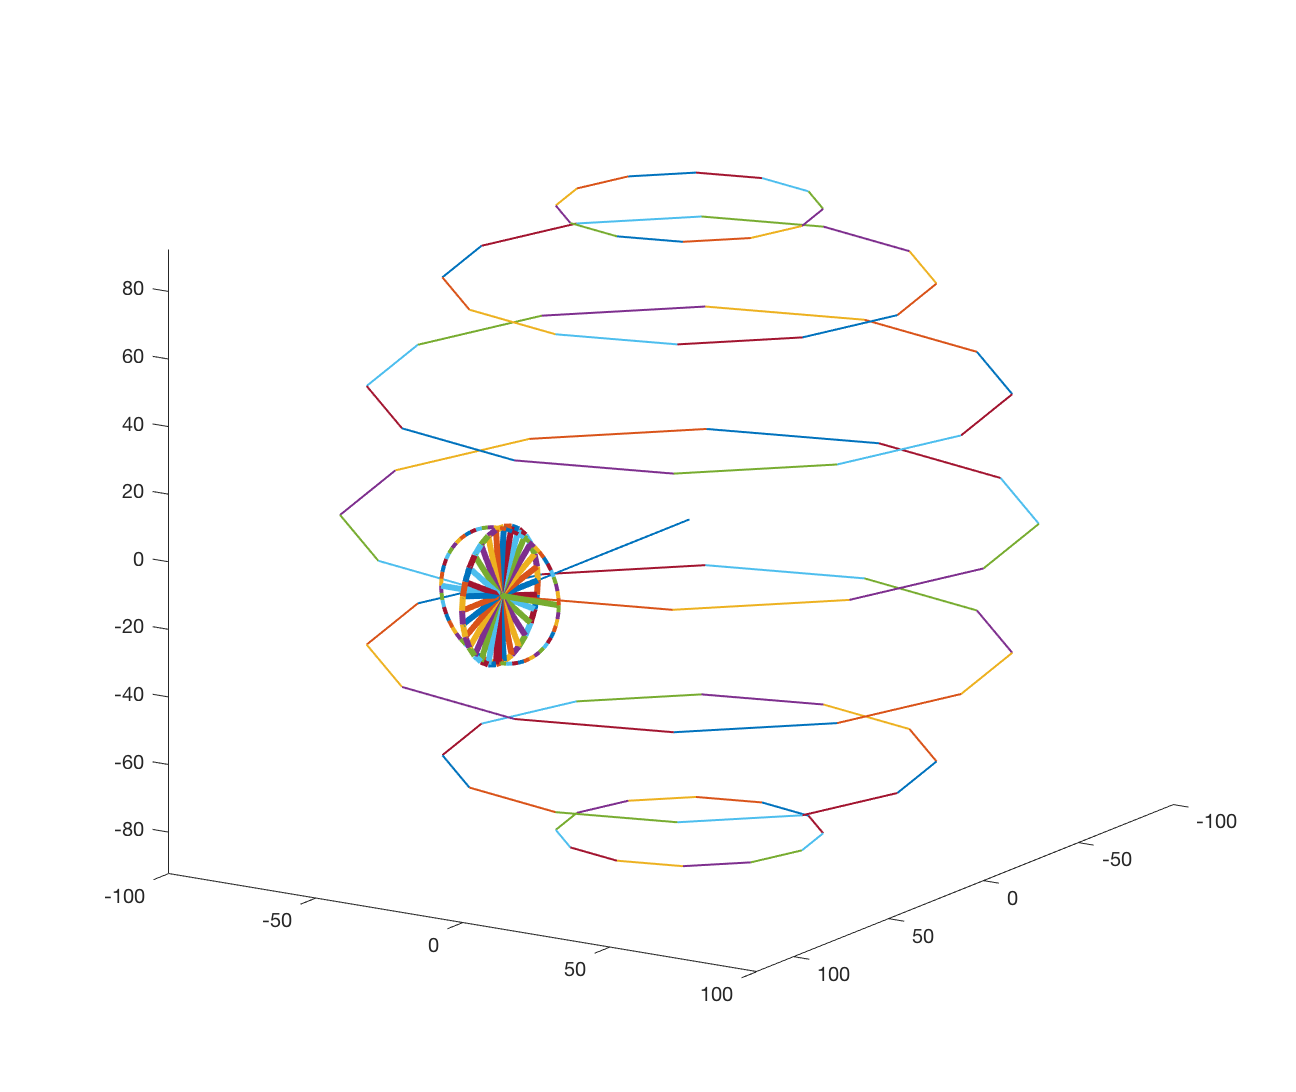
\includegraphics[width=0.7\textwidth]{gyrocompass_at_equator.png}
    		
    
    \end{figure}
    
\end{frame}
\begin{frame}{Gyrocompass}
    \begin{figure}
    		\centering
    		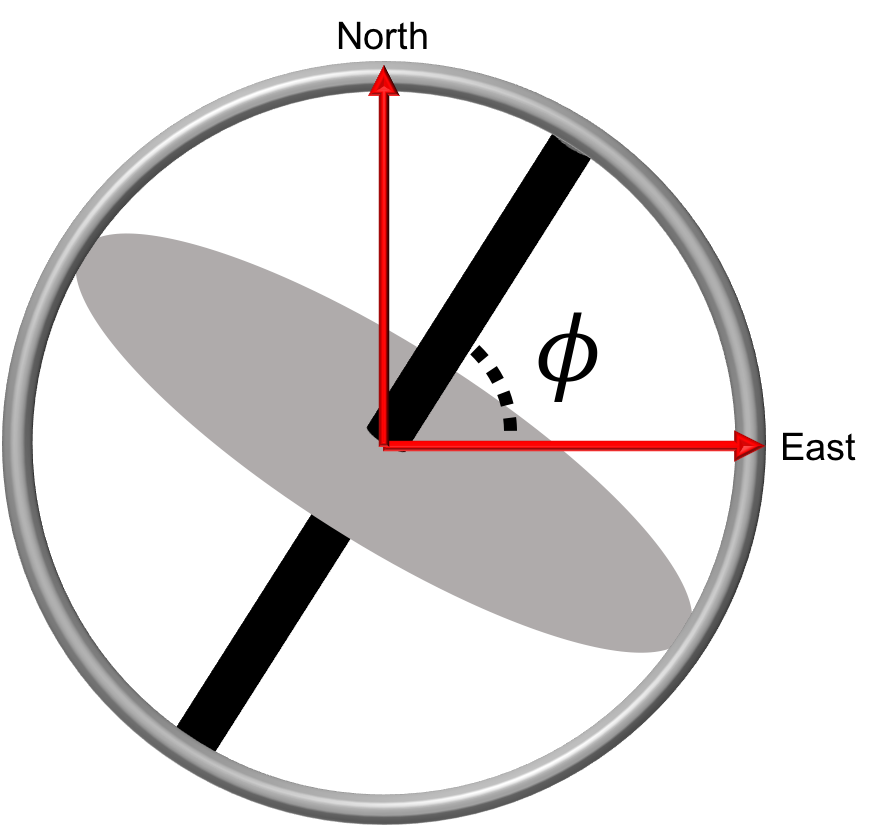
\includegraphics[width=0.55\textwidth]{define_phi.png}
  
    \end{figure}
\end{frame}

\begin{frame}{Gyrocompass}
    \begin{figure}
    	
    		\centering
    		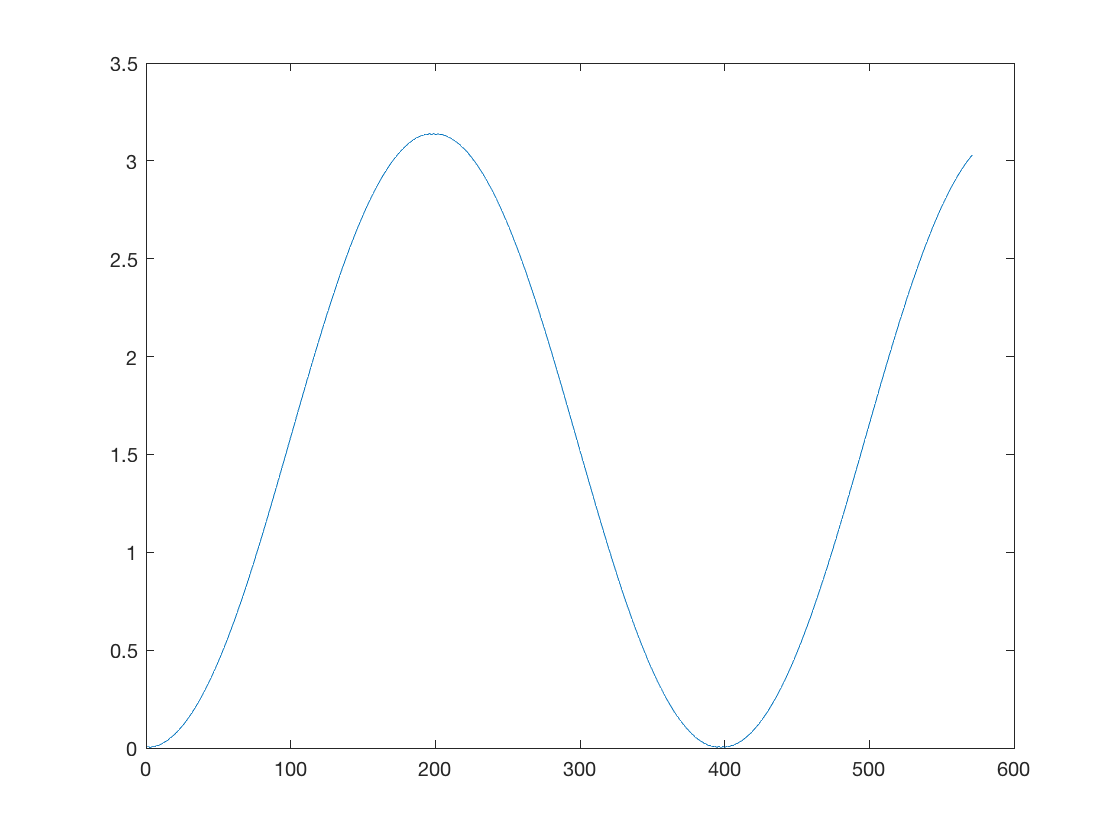
\includegraphics[width=0.89\textwidth]{L5000.png}
    		
    \end{figure}
\end{frame}



\end{document}
